\documentclass[11pt,letterpaper]{article}
\usepackage[lmargin=1in,rmargin=1in,tmargin=1in,bmargin=1in]{geometry}
\usepackage{../style/homework}
\usepackage{../style/commands}
\setbool{quotetype}{true} % True: Side; False: Under
\setbool{hideans}{false} % Student: True; Instructor: False

% -------------------
% Content
% -------------------
\begin{document}

\homework{6: Due 01/12}{I'm always thinking one step ahead, like a carpenter that makes stairs.}{Andy Bernard, The Office}

% Problem 1
\problem{10} A linear function is plotted below. Find the equation of this linear function. 
	\[
	\fbox{
	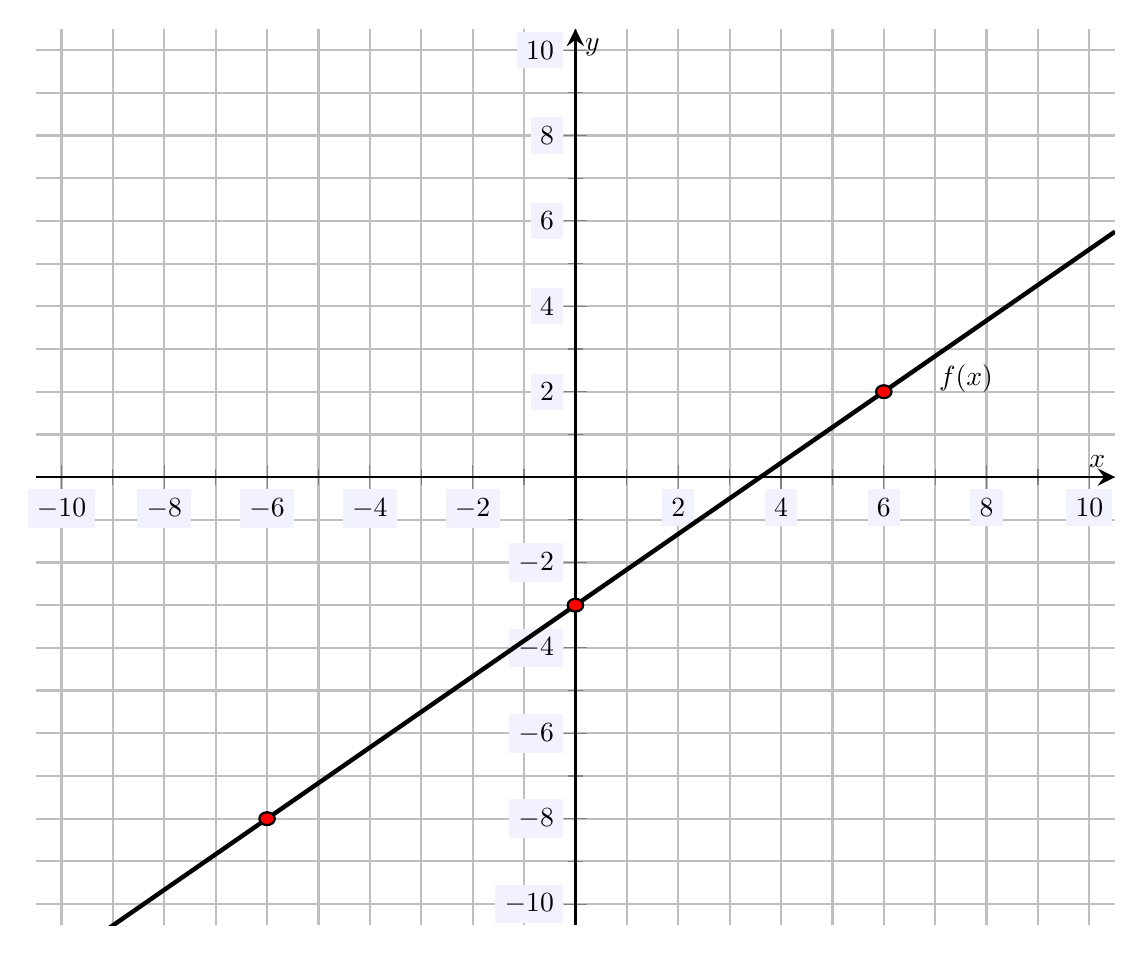
\begin{tikzpicture}[scale=2,every node/.style={scale=0.5}]
	\begin{axis}[
	grid=both,
	axis lines=middle,
	ticklabel style={fill=blue!5!white},
	xmin= -10.5, xmax=10.5,
	ymin= -10.5, ymax=10.5,
	xtick={-10,-8,-6,-4,-2,0,2,4,6,8,10},
	ytick={-10,-8,-6,-4,-2,0,2,4,6,8,10},
	minor tick = {-10,-9,...,10},
	xlabel=\(x\),ylabel=\(y\),
	]
	\node at (7.6,2.3) {$f(x)$};
	\addplot[thick, domain= -10.5:10.5] ({x},{5/6*x - 3});
	
	\draw[fill=red] (-6, -8) circle (0.15);
	\draw[fill=red] (0, -3) circle (0.15);
	\draw[fill=red] (6, 2) circle (0.15);
	\end{axis}
	\end{tikzpicture}
	}
	\] \pspace

\sol Because the line is not vertical, it has the form $y= mx + b$. We can see from the plot that the the points $(-6, -8)$, $(0, -3)$, and $(6, 2)$ are on the line. Using any two of them, we find the slope of the line:
	\[
	m= \dfrac{\Delta y}{\Delta x}= \dfrac{-3 - (-8)}{0 - (-6)}= \dfrac{-3 + 8}{0 + 6}= \dfrac{5}{6}
	\] 
Then we know $y= \frac{5}{6}x + b$. Because $(0, -3)$ is the $y$-intercept, we know that $b= -3$. Therefore, $y= \frac{5}{6}x - 3$. Alternatively, for example, because the line contains the point $(6, 2)$, the point $(6, 2)$ satisfies the equation of the line. But then $y= \frac{5}{6}x + b$ implies $2= \frac{5}{6} \cdot 6 + b= 5 + b$ so that $b= -3$. \pspace

Alternatively, we can see from the plot that the points $(0, -3)$ and $(6, 2)$ are on the line. Therefore, when $x$ increases by 6, $y$ increases by 5. Therefore, the slope is $m= \frac{\Delta y}{\Delta x}= \frac{5}{6}$. Because we know $y= mx + b$, it must be that $y= \frac{5}{6}x + b$. We can then find $b$ as above. 



\newpage



% Problem 2
\problem{10} Determine if the following pairs of lines are the same, perpendicular, parallel, or none of these. 
	\[
	\begin{aligned}
	\ell_1&: & y= \dfrac{3}{2}\,&x + 9 \\
	\ell_2&: & 9x - 6y&= 12
	\end{aligned}
	\] \pspace

\sol Solving for $y$ in the second equation, we find\dots
	\[
	\begin{aligned}
	9x - 6y&= 12 \\[0.3cm]
	-6y&= -9x + 12 \\[0.3cm]
	y&= \dfrac{3}{2}\,x - 2
	\end{aligned}
	\] 
Therefore, the lines are\dots
	\[
	\begin{aligned}
	\ell_1&: & y&= \dfrac{3}{2}\,x + 9 \\
	\ell_2&: & y&= \dfrac{3}{2}\,x - 2
	\end{aligned}
	\]
The slope of the first line is $m_1= \frac{3}{2}$ and the slope of the second line is $m_2= \frac{3}{2}$. Because $m_1= m_2$, either the lines are parallel are the same. But the $y$-intercept of the first line is $(0, 9)$ while the $y$-intercept of the second line is $(0, -2)$. Therefore, the lines are parallel, i.e. $\ell_1 \parallel \ell_2$. 



\newpage



% Problem 3
\problem{10} Determine if the following pairs of lines are the same, perpendicular, parallel, or none of these. 
	\[
	\begin{aligned}
	\ell_1&: & 2x - 3y&= 5 \\
	\ell_2&: & 6x + 5y&= -3
	\end{aligned}
	\] \pspace

\sol Solving for $y$ in the first equation, we find\dots
	\[
	\begin{aligned}
	2x - 3y&= 5 \\[0.3cm]
	-3y&= -2x + 5 \\[0.3cm]
	y&= \dfrac{2}{3}\,x - \dfrac{5}{3}
	\end{aligned}
	\]
Solving for $y$ in the second equation, we find\dots
	\[
	\begin{aligned}
	6x + 5y&= -3 \\[0.3cm]
	5y&= -6x - 3 \\[0.3cm]
	y&= -\frac{6}{5}\,x - \frac{3}{5}
	\end{aligned}
	\] 
Therefore, the lines are\dots
	\[
	\begin{aligned}
	\ell_1&: & y&= \dfrac{2}{3}\,x - \dfrac{5}{3} \\
	\ell_2&: & y&= -\dfrac{6}{5}\,x - \dfrac{3}{5}
	\end{aligned}
	\]
The slope of the first line is $m_1= \frac{2}{3}$ and the slope of the second line is $m_2= -\frac{6}{5}$. Because $m_1 \neq m_2$, the lines are not the same or parallel, so that they must intersect. Because the negative reciprocal of $m_1= \frac{2}{3}$ is $\frac{3}{2} \neq -\frac{6}{5}$. Therefore, the lines are not perpendicular. But then $\ell_1$ and $\ell_2$ are distinct lines that are not parallel and hence intersect (but not perpendicularly). 



\newpage



% Problem 4
\problem{10} Determine if the following pairs of lines are the same, perpendicular, parallel, or none of these. 
	\[
	\begin{aligned}
	\ell_1&: & y= -2x& + 7 \\
	\ell_2&: & -3x + 6y&= 15
	\end{aligned}
	\] \pspace

\sol Solving for $y$ in the second equation, we find\dots
	\[
	\begin{aligned}
	-3x + 6y&= 15 \\[0.3cm]
	6y&= 3x + 15 \\[0.3cm]
	y&= \dfrac{1}{2}\,x + \dfrac{5}{2}
	\end{aligned}
	\] 
Therefore, the lines are\dots
	\[
	\begin{aligned}
	\ell_1&: & y&= -2x + 7 \\
	\ell_2&: & y&= \dfrac{1}{2}\,x + \dfrac{5}{2}
	\end{aligned}
	\]
The slope of the first line is $m_1= -2$ and the slope of the second line is $m_2= \frac{1}{2}$. Because $m_1 \neq m_2$, the lines cannot be the same or parallel, so that they must intersect. Because the negative reciprocal of $m_1= -2= -\frac{2}{1}$ is $-\frac{1}{2}= m_2$. Therefore, the lines are perpendicular, i.e. $\ell_1 \perp \ell_2$. 



\newpage



% Problem 5
\problem{10} Find the equation of the line passing through the points $(6, 21)$ and $(-9, -19)$. \pspace

\sol Because the line is not vertical, we know that the line has the form $y= mx + b$. We first find the slope:
	\[
	m= \dfrac{\Delta y}{\Delta x}= \dfrac{21 - (-19)}{6 - (-9)}= \dfrac{21 + 19}{6 + 9}= \dfrac{40}{15}= \dfrac{8}{3}
	\]
Therefore, $y= \frac{8}{3}x + b$. Because the point $(6, 21)$ is on the line, it satisfies the equation of the line. Therefore, we know\dots
	\[
	\begin{aligned}
	y&= \dfrac{8}{3}x + b \\[0.3cm]
	21&= \dfrac{8}{3} \cdot 6 + b \\[0.3cm]
	21&= 8(2) + b \\[0.3cm]
	21&= 16 + b \\[0.3cm]
	b&= 5
	\end{aligned}
	\]
Therefore, the equation of the line is $y= \frac{8}{3}x + 5$. 



\newpage



% Problem 6
\problem{10} Find the equation of the line perpendicular to $y= 4 - 5x$ that passes through the point $(3, -1)$. \pspace

\sol Because the line is not vertical, we see that it has the form $y= mx + b$. The line $y= 4 - 5x$ has slope $-5$. Because our line is perpendicular to the line $y= 4 - 5x$, our line must have slope equal to the negative reciprocal of $-5$, which is $-(\frac{1}{-5})= \frac{1}{5}$. Therefore, $m= \frac{1}{5}$ so that $y= \frac{1}{5}x + b$. Because the line contains the point $(3, -1)$, the point satisfies the equation of the line. Therefore, we know\dots
	\[
	\begin{aligned}
	y&= \dfrac{1}{5}x + b \\[0.3cm]
	-1&= \dfrac{1}{5} \cdot 3 + b \\[0.3cm]
	-1&= \dfrac{3}{5} + b \\[0.3cm]
	b&= -1 - \dfrac{3}{5} \\[0.3cm] 
	b&= -\dfrac{5}{5} - \dfrac{3}{5} \\[0.3cm]
	b&= -\dfrac{8}{5}
	\end{aligned}
	\]
Therefore, the equation of the line $y= \frac{1}{5} x - \frac{8}{5}= \frac{x - 8}{5}$. 



\newpage



% Problem 7
\problem{10} Find the equation of the line parallel to the line $x= -5$ containing the point $(4, 19)$. \pspace

\sol The line $x= -5$ is a vertical line. Because our line is parallel to this line, it must also be vertical, i.e. our line has the form $x= M$ for some $M$. Because our line passes through the point $(4, 19)$, we know that we must have $x= 4$. 



\newpage



% Problem 8
\problem{10} Sunita works at an advertising firm. Upon hire, she was paid a \$5,000 signing bonus. The company pays her a yearly salary of \$63,000. 
        \begin{enumerate}[(a)]
        \item Write a function which gives the amount of money Sunita has been paid by the company in $t$ years. 
        \item What is the slope and $y$-intercept for the function in (a)? Interpret both of these in the problem context. 
        \item Find the amount of money Sunita has been paid in 5~years.
        \item How many years until Sunita has been paid a total of \$200,000. 
        \end{enumerate} \pspace

\sol
\begin{enumerate}[(a)]
\item Let $P(t)$ be the amount Sunita has been paid after $t$ years. Because she is paid \$63,000 each year, after $t$ years, she has been paid a total salary of $63000t$. But she was also paid a signing bonus of $5000$. Therefore, $P(t)= 63000t + 5000$. \pspace

\item We know that $P(t)$ is linear because Sunita receives a constant salary of \$63000/year. Moreover, $P(t)= 63000t + 5000$ is a linear function because it has the form $y= mx + b$. We then know that $m= 63000$ and $b= 5000$. Interpreting $m= 63000= \frac{63000}{1}$ as $\frac{\Delta y}{\Delta x}$, we have $\Delta x= 1$ and $\Delta y= 63000$ and using the fact that $x$ has units of years and $y$ has units of dollars, we see that every year Sunita is paid \$63,000, i.e. the slope represents her yearly salary of \$63,000. The $y$-intercept is $(0, 5000)$, i.e. when $t= 0$ we know that $P(0)= 5000$. We know that $t= 0$ is the time of hire. Therefore, Sunita must have been paid \$5,000 upon hire, i.e. the $y$-intercept represents Sunita's signing bonus. \pspace

\item Although, Sunita will only receive a salary of \$63,000 in 5~years, the total amount of money she has been paid will be $P(5)$, which is\dots
	\[
	P(5)= 63000(5) + 5000= 315000 + 5000= \$320,000
	\] \pspace

\item When Sunita has been paid a total of \$200,000, this is a time $t$ such that $P(t)= 200000$. But then\dots
	\[
	\begin{aligned}
	P(t)&= 200000 \\[0.3cm]
	63000t + 5000&= 200000 \\[0.3cm]
	63000t&= 195000 \\[0.3cm]
	t&= 3.09524 \text{ years}
	\end{aligned}
	\]
Therefore, she would have been paid a total of \$200,000 between her third and fourth year working at the firm. One might say that she will have been paid at least \$200,000 after her third year at the firm (or by the start of her fourth year at the firm). 
\end{enumerate}



\newpage



% Problem 9
\problem{10} A tour bus company charged a group of 30~people a total of \$180 for a tour. The following week, they charged a group of 50~people \$220.
        \begin{enumerate}[(a)]
        \item Find a linear function, $C(p)$, for the total cost for a tour for a group of size $p$. 
        \item What is the slope of $C(p)$? Interpret the slope in context. 
        \item What is the $y$-intercept? Does it have meaning in this context? Explain. 
        \item Estimate much would the company charge for a group of 60~people.
        \item If you only had \$570, what would you estimate the largest group you could take on the tour?
        \end{enumerate} \pspace

\sol
\begin{enumerate}[(a)]
\item We know $C(30)= 180$ and $C(50)= 220$, i.e. that the graph of $C(p)$ contains the points $(30, 180)$ and $(50, 220)$. Because $C(p)$ is not a vertical line, we know that $C(p)= mp + b$. The slope of $C(p)$ must be\dots
	\[
	m= \dfrac{180 - 220}{30 - 50}= \dfrac{-40}{-20}= 2
	\]
But then $C(p)= 2p + b$. Because $(30, 180)$ is on the graph of $C(p)$, it satisfies the equation for $C(p)$. Then we know\dots
	\[
	\begin{aligned}
	C(p)&= 2p + b \\
	C(30)&= 2(30) + b \\
	180&= 60 + b \\
	b&= 120
	\end{aligned}
	\]
Therefore, $C(p)= 2p + 120$. \pspace

\item Because $C(p)= 2p + 120$ has the form $y= mx + b$, we know that $m= 2= \frac{2}{1}$. Interpreting this as $\frac{\Delta y}{\Delta x}$, we have $\Delta x= 1$ and $\Delta y= 2$. Using the fact that $x$ has units of people and $y$ has units of dollars, we interpret the slope as the fact that the company charges \$2 per person. \pspace

\item Because $C(0)= 2(0) + 120= 120$, we know that the $y$-intercept for $C(p)$ is $(0, 120)$, i.e. when $p= 0$, we know that $C(0)= \$120$. This is a charge of \$120 for a tour with no people---which is nonsensical. However, we can interpret this as a fee charged to give a tour at all, i.e. a service charge or booking charge of \$120. \pspace

\item This is $C(60)$, which is $C(60)= 2(60) + 120= 120 + 120= \$240$. \pspace

\item We want a number of people, $p$, so that $C(p)= 570$. But then $2p + 120= 570$, which implies that $2p= 450$. Therefore, we know that $p= 225$. But then the largest number of people you could bring on the tour would be 225~people. 
\end{enumerate}



\newpage



% Problem 10
\problem{10} A used car was purchased for \$7,500. Each year, the car loses \$1,200 in value.
        \begin{enumerate}[(a)]
        \item Find a function, $V(t)$, which gives the value, $V$, for the car after $t$ years.
        \item What does the slope of $V(t)$ represent?
        \item What does the $y$-intercept of $V(t)$ represent?
        \item What is the car worth in 3~years?
        \item How long until the car is essentially worthless? 
        \end{enumerate} \pspace

\sol
\begin{enumerate}[(a)]
\item Because the rate of depreciation of the vehicle is constant, we know that $V(t)$ is linear. After $t$ years, the car has lost $1200t$ dollars in value. But because the car was initially worth $7500$, we know that $V(t)= 7500 - 1200t$. \pspace

\item Because $V(t)= 7500 - 1200t$ has the form $y= mx + b$, we know that $m= -1200= \frac{-1200}{1}$. Interpreting this as $\frac{\Delta y}{\Delta x}$, we have $\Delta x= 1$ and $\Delta y= -1200$. Using the fact that $x$ has units of years and $y$ has units of dollars, we interpret the slope as the fact that the car loses \$1,200 in value each year. \pspace

\item We know that the $y$-intercept occurs when $t= 0$ and that $V(0)= 7500 - 1200(0)= 7500 - 0= \$7,500$. Because $V(0)$ represents the value of the car at $t= 0$, i.e. at the time of purchase, the $y$-intercept must represent the initial value of the car. \pspace

\item This is $V(3)$, which is $V(3)= 7500 - 1200(3)= 7500 - 3600= \$3,900$. \pspace

\item The car is worthless when it has value \$0. But then this is a time when $V(t)= 0$. But then we have\dots
	\[
	\begin{aligned}
	V(t)&= 0 \\[0.3cm]
	7500 - 1200t&= 0 \\[0.3cm]
	7500&= 1200t \\[0.3cm]
	t&= 6.25 \text{ years}
	\end{aligned}
	\]
Therefore, the car has no value after 6~years and 3~months. 
\end{enumerate}


\end{document}